%include part: see main.beamer.tex and main.article.tex
%include common packages and settings
\usepackage{etex} %эта магическая херь избавляет от переполнения регистров TeX а!!!

\mode<article>{\usepackage{fullpage}}
\mode<presentation>{
    \usetheme{Madrid} %%Boadilla,Madrid,AnnArbor,CambridgeUS,Malmoe,Singapore,Berlin
    \useoutertheme{shadow}
} 

\usepackage[utf8]{inputenc}
\usepackage[russian]{babel}
\usepackage{indentfirst}
\usepackage{graphicx}

\usepackage{amsmath}
\usepackage{amsfonts}
\usepackage{amsthm}
\usepackage{algorithm}
\usepackage{algorithmic}

\usepackage[all]{xy}

\date{Лекция по дисциплине <<дискретная математика>>\\(\today)}
\author[М.~М.~Шихов]{Михаил Шихов \\ \texttt{\underline{m.m.shihov@gmail.com}}}

%для рисования графов пакетом xy-pic
\entrymodifiers={++[o][F-]}

%для псевдокода алгоритмов (algorithm,algorithmic)
\renewcommand{\algorithmicrequire}{\textbf{Вход:}}
\renewcommand{\algorithmicensure}{\textbf{Выход:}}
\renewcommand{\algorithmiccomment}[1]{// #1}
\floatname{algorithm}{Псевдокод}



\title[Графы]{Основы теории графов}


\begin{document}

%титул и содержание статьи
\mode<article>{\maketitle\tableofcontents}

%титул и содержание презентации
\frame<presentation>{\titlepage}
\begin{frame}<presentation>
    \frametitle{Содержание}
    \tableofcontents
\end{frame}


\section{История}

\subsection{Задача о Кёнигсбергских мостах}

История графов началась с головоломок. Первым упоминанием считается 1736 г., когда Леонард Эйлер решил задачу о Кёнигсбергских мостах, используя граф.

\begin{frame}
    \frametitle{Задача о Кёнигсбергских мостах (1736 г.)}
    
    Река Прегель (Преголя) делила Кёнигсберг на четыре главные части: Альтштадт ($A$), Форштадт ($B$), Кнайпхоф ($C$) и Ломзе ($D$). Части соединены друг с другом семью мостами. Возможно ли составить такой маршрут, чтобы пройти по каждому мосту только один раз и вернуться в исходную точку?
    \[
        \begin{tabular}{ccc}
            \raisebox{-1.\height}{
                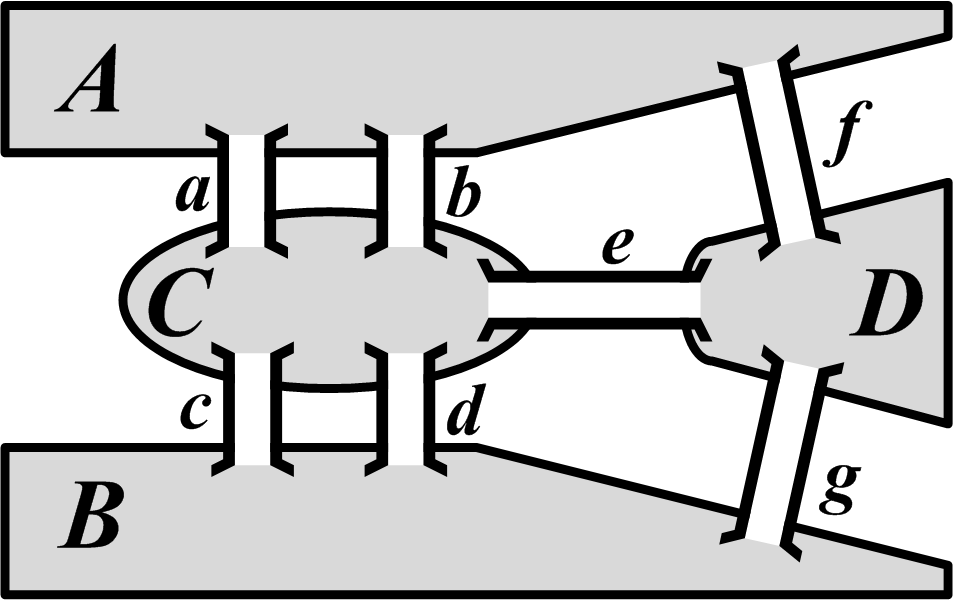
\includegraphics[width=0.3\textwidth]{fig/kenigsberg.png}
            }
            &&
            {\xymatrix{
                A \ar@{-}@/^/[d]^b \ar@{-}@/_/[d]_a \ar@{-}@/^/[dr]^f
                    &*{}
                        \\
                C \ar@{-}[r]^e
                    &D
                        \\
                B \ar@{-}@/^/[u]^c \ar@{-}@/_/[u]_d \ar@{-}@/_/[ur]_g
                    &*{}
            }}
        \end{tabular}
    \]
\end{frame}


\section{Основные определения}

\subsection{Графы}

\begin{frame}
    \frametitle{Определение}
    
    \begin{definition}
        Граф $G$ --- это совокупность $G=\langle V,P\rangle$ \alert{множества} вершин $V$ и \alert{набора} отрезков $P$, соединяющих пары вершин. 
    \end{definition}

    \begin{itemize}
        \item Отдельный отрезок может быть представлен упорядоченной $(a,b)$ (или неупорядоченной $[a,b]$) парой, где $a,b\in V$.
    
        \item В общем случае, в \alert{наборе} $P$ могут присутствовать несколько одинакового вида пар $(a,b)$.
    \end{itemize}
\end{frame}

Отрезок $[a,a]$, соединяющий вершину $a$ с ней самой, называется \emph{петлей}.

Неупорядоченная пара вершин $[a,b]$ (т.е. $[a,b]=[b,a]$) называется \emph{ребром}, а граф, содержащий только ребра называется \emph{неориентированным}.

Упорядоченная пара вершин $(a,b)$ (т.е. $(a,b)\neq(b,a)$) называется \emph{дугой}, а граф, содержащий только дуги называется \emph{ориентированным} или \emph{орграфом}. Дуга изображается стрелкой.

Если набор $P$ содержит несколько одинаковых отрезков-пар, то такие пары называются \emph{кратными}, а граф называется \emph{мультиграфом}.

%uncover работает для вершин, а only работает для стрелок!!!
\begin{frame}
    \frametitle{Виды графов}
    \[
        G=\langle V,P\rangle
    \]
    \begin{columns}
        \column{.3\textwidth}
            \begin{block}{Неориентированный}
                \[
                    {\xymatrix{
                        a \ar@{-}[r] \ar@{-}[d]
                            &c \ar@{-}[d] \ar@{-}@(u,r)[]
                                \\
                        b \ar@{-}[ur] \ar@{-}[r]
                            &d
                    }}
                \]
                $[c,d]$ --- \alert{ребро}
            \end{block}
        
        \column{.3\textwidth}
            \begin{block}{Ориентированный}
                \[
                    {\xymatrix{
                        a \ar@{->}[r]
                            &c \ar@{->}@(u,r)[]
                                \\
                        b  \ar@{->}[u] \ar@{->}[ur] \ar@{->}[r]
                            &d \ar@{->}[u]
                    }}
                \]
                $(d,c)$ --- \alert{дуга}
            \end{block}
        \column{.3\textwidth}
            \begin{block}{Мультиграф}
            
                \[
                    {\xymatrix{
                        a \ar@{-}[r] \ar@{-}@/^/[d]
                            &c \ar@{-}[d] \ar@{-}@(u,r)[]
                                \\
                        b \ar@{-}[ur] \ar@{-}@/^/[r] \ar@{-}@/^/[u]
                            &d \ar@{-}@/^/[l]
                    }}
                \]
                $[c,c]$ --- \alert{петля}
            \end{block}
    \end{columns}
\end{frame}

Если задана функция $f:V\to M$ и/или $f:P\to M$, то множество $M$ называтется множеством \emph{пометок}, а граф называется \emph{помеченным}\footnote{Граф на рисунке \ref{fig:graph:kenigsberg} --- помеченный} (или \emph{нагруженным}). Пометка на изображении графа пишется над соответствующей вершиной или отрезком. Если пометка представляет собой число (или элемент упорядоченного множества), то она называется \emph{весом}, а граф --- \emph{взвешенным}.


\begin{frame}
    \frametitle{Помеченные (нагруженные) графы}

    \[
        G=\langle V,P\rangle,f_1:V\to M_1,f_2:P\to M_2
    \]    
    \begin{columns}
        \column{.3\textwidth}
            \begin{block}{Помеченный граф}
                \[
                    {\xymatrix{
                        \ar@{-}[r]^{a}
                            &\ar@{-}@(u,r)[]|-{b}
                                \\
                        \ar@{-}[u]^{c} \ar@{-}[ur]|-{d} \ar@{-}[r]_{e}
                            &\ar@{-}[u]_{f}
                    }}
                \]
            \end{block}
        \column{.3\textwidth}
            \begin{block}{Взвешенный орграф}
                \[
                    {\xymatrix{
                        \ar@{->}[r]^{1}
                            &\ar@{->}@(u,r)[]|-{0}
                                \\
                        \ar@{->}[u]^{2} \ar@{->}[ur]|-{3} \ar@{->}[r]_{4}
                            &\ar@{->}[u]_{5}
                    }}
                \]
            \end{block}
        \column{.3\textwidth}
            \begin{block}{Взвешенный орграф}
                \[
                    {\xymatrix{
                        a \ar@{->}[r]^{1}
                            &c \ar@{->}@(u,r)[]|-{0}
                                \\
                        b \ar@{->}[u]^{2} \ar@{->}[ur]|-{3} \ar@{->}[r]_{4}
                            &d \ar@{->}[u]_{5}
                    }}
                \]
            \end{block}
    \end{columns}
\end{frame}


\subsection{Элементы графов и их свойства}

Вершины, соединенные одним ребром, называются \emph{смежными}. Ребра, имеющие общую вершину, также называются \emph{смежными}. Ребро \emph{инцидентно} вершинам, которые оно соединяет, и вершины также \emph{инцидентны} этому ребру.

\begin{frame}
    \frametitle{Смежность и инцидентность}

    \[
        {\xymatrix{
            \uncover<1,2,3,4,6>{1}
            \ar@{-}[r]
                &\uncover<1,6>{3}
                \ar@{-}@(u,r)[]
                    \\
            \uncover<1,2,3,4,5,6>{2}
            \only<1,5,6>{\ar@{-}[u]}\only<2,3,4>{\ar@{:}[u]} 
            \ar@{-}[ur] 
            \only<1,2,4,6>{\ar@{-}[r]}\only<3,5>{\ar@{:}[r]}
                &\uncover<1,3,5,6>{4}
                \ar@{-}[u]
        }}
    \]
    
    \begin{itemize}
        \item<2,6> Вершины $1$ и $2$ --- \alert<2>{смежны}.
        \item<3,6> Ребра $[1,2]$ и $[2,4]$ --- \alert<3>{смежны}.
        \item<4,6> Ребро $[1,2]$ \alert<4>{инцидентно} вершинам $1$ и $2$.
        \item<5,6> Вершины $2$ и $4$ \alert<5>{инцидентны} ребру $[2,4]$.
    \end{itemize}
    \uncover<6>{Смежными бывают однородные элементы, а инцидентными разнородные.}
\end{frame}

\emph{Степенью} вершины называется число ребер, инцидентных этой вершине. В орграфах различают полустепени исхода (количество исходящих дуг) и захода (количество входящих дуг).

\begin{frame}
    \frametitle{Степени вершин}

    \begin{columns}
        \column{.47\textwidth}
            \begin{block}{Неориентированный граф}
                \[
                    {\xymatrix{
                        a   \only<1,2,4>{\ar@{-}[r]}\only<3>{\ar@{:}[r]}
                            \only<1,3,4>{\ar@{-}[d]}\only<2>{\ar@{:}[d]}
                            &c  \only<1,2,4>{\ar@{-}[d]}\only<3>{\ar@{:}[d]}
                                \only<1,2,4>{\ar@{-}@(u,r)[]}\only<3>{\ar@{:}@(u,r)[]}
                                \\
                        b   \only<1,4>{\ar@{-}[ur]}\only<2,3>{\ar@{:}[ur]}  
                            \only<1,3,4>{\ar@{-}[r]}\only<2>{\ar@{:}[r]}
                            &d
                    }}
                \]
                \begin{itemize}
                    \item<2,4> \alert<2>{Степень} вершины $b$=$3$;
                    \item<3,4> \alert<3>{Степень} вершины $c$=$4$.
                \end{itemize}
                \uncover<4>{Сумма степеней всех вершин графа в два раза больше количества ребер.}
            \end{block}
        
        \column{.47\textwidth}
            \begin{block}{Ориентированный граф}
                \[
                    {\xymatrix{
                        a \ar@{->}[r]
                            &c \ar@{->}@(u,r)[]
                                \\
                        b   \only<1,3,4>{\ar@{->}[u]}\only<2>{\ar@{:>}[u]}
                            \only<1,2,4>{\ar@{<-}[ur]}\only<3>{\ar@{<:}[ur]}
                            \only<1,3,4>{\ar@{->}[r]}\only<2>{\ar@{:>}[r]}
                            &d \ar@{->}[u]
                    }}
                \]
                \begin{itemize}
                    \item<2,4> Полустепень \alert<2>{исхода} $b$=$2$;
                    \item<3,4> Полустепень \alert<3>{захода} $b$=$1$.
                \end{itemize}                
                \uncover<4>{Сумма соответствующих полустепеней всех вершин графа равна количеству дуг.}
            \end{block}
    \end{columns}
\end{frame}

Граф называется \emph{полным}, если между любыми его вершинами существует ребро. В полном графе с $n$ вершинами число ребер $m=\frac{n(n-1)}{2}$. \emph{Дополнение} графа до полного содержит все ребра полного графа, не принадлежащие исходному графу.

\emph{Подграфом} называется граф, в который входит лишь часть вершин исходного графа и часть его ребер, эти вершины соединяющих.

\begin{frame}
    \frametitle{Подграф, полный граф и дополнение графа}

    \begin{columns}
        \column{.3\textwidth}
            \begin{block}{$G=\langle V,P\rangle,n=5$}
                \[
                    {\xymatrix{
                        *{} 
                            & \ar@{-}[dr] \ar@{-}[dl] 
                                &*{}
                                    \\
                        {} 
                            &*{}
                                & \ar@{-}[d] 
                                    \\
                        \ar@{-}[u] 
                            &*{}
                                & \ar@{-}[ll]
                    }}
                \]
            \end{block}
        
        \column{.3\textwidth}
            \begin{block}{Полный граф $n=5$}
                \[
                    {\xymatrix{
                        *{} 
                            & \ar@{-}[dr] \ar@{-}[ddr] \ar@{-}[ddl] \ar@{-}[dl] 
                                &*{}
                                    \\
                        {} 
                            &*{}
                                & \ar@{-}[d] \ar@{-}[dll] \ar@{-}[ll] 
                                    \\
                        \ar@{-}[u] 
                            &*{}
                                & \ar@{-}[ll] \ar@{-}[ull] 
                    }}
                \]
            \end{block}
        \column{.3\textwidth}
            \begin{block}{$\overline{G}, n=5$}
                \[
                    {\xymatrix{
                        *{} 
                            & \ar@{-}[ddr] \ar@{-}[ddl] 
                                &*{}
                                    \\
                        {} 
                            &*{}
                                & \ar@{-}[dll] \ar@{-}[ll] 
                                    \\
                        {} 
                            &*{}
                                & \ar@{-}[ull] 
                    }}
                \]
            \end{block}
    \end{columns}
    
    Количество ребер полного графа 
    \[
        m=\frac{n(n-1)}{2}.
    \]
\end{frame}


\subsection{Маршруты в графах}

Последовательность 
\begin{equation}
    \label{eq:graph:path}
    v_1,p_1,v_2,p_2,\ldots,p_{n},v_{n+1},
\end{equation}
где $v_1,v_2,\ldots,v_{n+1}\in V$, $p_1,p_2,\ldots,p_{n}\in P$ и любые два соседних элемента инцидентны (т.е. $p_i=(v_i,v_{i+1}), 1\leq i\leq n$) называется \emph{$(v_1,v_{n+1})$-маршрутом}. $n$ --- число отрезков $p_i$ маршрута называется его \emph{длиной}.

\begin{frame}
    \frametitle{Маршрут $(v_1,v_{n+1})$}
    \framesubtitle{$v_1,p_1,v_2,p_2,\ldots,p_{n},v_{n+1}$}

    \begin{columns}
        \column{.4\textwidth}
            \begin{block}{$G=\langle V,P\rangle,n=5$}
                \[
                    {\xymatrix{
                        1 \ar@{-}[dd]_{a} \ar@{-}[rr]^{d} \ar@{-}[dr]_{b}
                            &*{}
                                &4 \ar@{-}[dd]^{h}
                                    \\
                        *{} 
                            &3 \ar@{-}[ur]_{f} \ar@{-}[dr]^{g}
                                &*{}
                                    \\
                        2  \ar@{-}[ur]^{c} \ar@{-}[rr]_{e}
                            &*{}
                                &5
                    }}
                \]
            \end{block}
        
        \column{.5\textwidth}
            \begin{block}{Маршрут $(1,5)$ \\ $1,b,3,c,2,a,1,b,3,g,5$}
                \[
                    {\xymatrix{
                        1 \ar@{:}[dd]_{a} \ar@{-}[rr]^{d} \ar@{:}[dr]_{b}
                            &*{}
                                &4 \ar@{-}[dd]^{h}
                                    \\
                        *{} 
                            &3 \ar@{-}[ur]_{f} \ar@{:}[dr]^{g}
                                &*{}
                                    \\
                        2  \ar@{:}[ur]^{c} \ar@{-}[rr]_{e}
                            &*{}
                                &5
                    }}
                \]
            \end{block}
    \end{columns}
\end{frame}

Если все отрезки маршрута (кроме, возможно $p_1$ и $p_{n-1}$) различны, то он называется \emph{цепью}. Если все вершины маршрута (кроме, возможно $v_1$ и $v_{n+1}$) различны (а значит и отрезки), то маршрут называется \emph{простой} цепью. В орграфе цепь называется \emph{путем}.

\begin{frame}
    \frametitle{Цепь и путь}

    \begin{columns}
        \column{.45\textwidth}
            \begin{block}{Цепь $(1,2)$\\$1,b,3,g,5,h,4,f,3,c,2$}
                \[
                    {\xymatrix{
                        1 \ar@{-}[dd]_{a} \ar@{-}[rr]^{d} \ar@{:}[dr]_{b}
                            &*{}
                                &4 \ar@{:}[dd]^{h}
                                    \\
                        *{} 
                            &3 \ar@{:}[ur]_{f} \ar@{:}[dr]^{g}
                                &*{}
                                    \\
                        2  \ar@{:}[ur]^{c} \ar@{-}[rr]_{e}
                            &*{}
                                &5
                    }}
                \]
            \end{block}
        
        \column{.45\textwidth}
            \begin{block}{Путь $(1,4)$\\$1,b,3,g,5,e,2,c,3,f,4$}
                \[
                    {\xymatrix{
                        1 \ar@{<-}[dd]_{a} \ar@{<-}[rr]^{d} \ar@{:>}[dr]_{b}
                            &*{}
                                &4 \ar@{<-}[dd]^{h}
                                    \\
                        *{} 
                            &3 \ar@{:>}[ur]_{f} \ar@{:>}[dr]^{g}
                                &*{}
                                    \\
                        2  \ar@{:>}[ur]^{c} \ar@{<:}[rr]_{e}
                            &*{}
                                &5
                    }}
                \]
            \end{block}
    \end{columns}    
\end{frame}

\begin{frame}
    \frametitle{Простая цепь и простой путь}

    \begin{columns}
        \column{.45\textwidth}
            \begin{block}{Простая цепь $(1,2)$\\$1,b,3,g,5,e,2$}
                \[
                    {\xymatrix{
                        1 \ar@{-}[dd]_{a} \ar@{-}[rr]^{d} \ar@{:}[dr]_{b}
                            &*{}
                                &4 \ar@{-}[dd]^{h}
                                    \\
                        *{} 
                            &3 \ar@{-}[ur]_{f} \ar@{:}[dr]^{g}
                                &*{}
                                    \\
                        2  \ar@{-}[ur]^{c} \ar@{:}[rr]_{e}
                            &*{}
                                &5
                    }}
                \]
            \end{block}
        
        \column{.45\textwidth}
            \begin{block}{Простой путь $(1,4)$\\$1,b,3,g,5,h,4$}
                \[
                    {\xymatrix{
                        1 \ar@{<-}[dd]_{a} \ar@{<-}[rr]^{d} \ar@{:>}[dr]_{b}
                            &*{}
                                &4 \ar@{<:}[dd]^{h}
                                    \\
                        *{} 
                            &3 \ar@{->}[ur]_{f} \ar@{:>}[dr]^{g}
                                &*{}
                                    \\
                        2  \ar@{->}[ur]^{c} \ar@{<-}[rr]_{e}
                            &*{}
                                &5
                    }}
                \]
            \end{block}
    \end{columns}
\end{frame}

Замкнутая ($v_1=v_n$) цепь называется \emph{циклом}. Замкнутая простая цепь называется \emph{простым} циклом. В орграфе цикл называется \emph{контуром}.

\begin{frame}
    \frametitle{Цикл и контур}

    \begin{columns}
        \column{.45\textwidth}
            \begin{block}{Цикл \\$1,d,4,h,5,e,2,a,1$}
                \[
                    {\xymatrix{
                        1 \ar@{:}[dd]_{a} \ar@{:}[rr]^{d} \ar@{-}[dr]_{b}
                            &*{}
                                &4 \ar@{:}[dd]^{h}
                                    \\
                        *{} 
                            &3 \ar@{-}[ur]_{f} \ar@{-}[dr]^{g}
                                &*{}
                                    \\
                        2  \ar@{-}[ur]^{c} \ar@{:}[rr]_{e}
                            &*{}
                                &5
                    }}
                \]
            \end{block}
        
        \column{.45\textwidth}
            \begin{block}{Контур\\$1,b,3,g,5,e,2,c,3,f,4,d,1$}
                \[
                    {\xymatrix{
                        1 \ar@{<-}[dd]_{a} \ar@{<:}[rr]^{d} \ar@{:>}[dr]_{b}
                            &*{}
                                &4 \ar@{<-}[dd]^{h}
                                    \\
                        *{} 
                            &3 \ar@{:>}[ur]_{f} \ar@{:>}[dr]^{g}
                                &*{}
                                    \\
                        2  \ar@{:>}[ur]^{c} \ar@{<:}[rr]_{e}
                            &*{}
                                &5
                    }}
                \]
            \end{block}
    \end{columns}    
    Циклы и контуры также могут быть \alert{простыми}, если все проходимые вершины различны.
\end{frame}

\section{Способы задания графов}

Существует множество способов задать граф:
\begin{itemize}
    \item аналитически;
    \item матрицей инцидентности;
    \item матрицей смежности;
    \item списком смежности.
\end{itemize}

Граф $G=\langle V,P\rangle$ можно задать аналитически, перечислив множество вершин $V$ и набор отрезков $P$.

Пусть $n=|V|$ --- количество вершин, а $m=|P|$ --- количество отрезков. 

Элементы \emph{матрицы инцидентности} $[G]_{n\times m}$ неориентированного графа определяются так:
\[
    [G]_{i,j}=
    \begin{cases}
        1, &\text{если вершина $v_i\in V$ инцидентна ребру $p_j\in P$},\\
        0, &\text{в противном случае.}
    \end{cases}
\]

В каждом $j$-м столбце матрицы по две $1$, если $p_j$ не петля, и одна в противном случае. 

Для орграфа элементы \emph{матрицы инцидентности} $[G]_{n\times m}$ определяются так:
\[
    [G]_{i,j}=
    \begin{cases}
         1, &\text{если вершина $v_i\in V$ --- начало дуги $p_j\in P$},\\
        -1, &\text{если вершина $v_i\in V$ --- конец дуги $p_j\in P$},\\
         0, &\text{в противном случае.}
    \end{cases}
\]

\emph{Матрица смежности вершин} $[G]_{n\times n}$:
\[
    [G]_{i,j}=
    \begin{cases}
         1, &\text{если $(v_i,v_j)\in P$},\\
         0, &\text{в противном случае.}
    \end{cases}
\]

Для мультиграфа вместо $1$ указывается количество кратных отрезков $(v_i,v_j)$.

Для представления графов в компьютерах наиболее часто используется \emph{список смежности вершин} 
\[
    \{v\mapsto \{v_s|v_s\in V,(v,v_s)\in P\}|v\in V\},
\]
для каждой вершины $v$ определяющий множество смежных с ней вершин $v_s$.

\subsection{Пример}

\begin{frame}
    \frametitle{Основные способы задания графа}
    
    \begin{columns}
        \column{.2\textwidth}
            \begin{block}{Граф}
                \[
                    {\xymatrix{
                        a \ar@{->}[r]^2
                            &b
                                \\
                        c \ar@{->}[r]_5 \ar@{->}[ur]^3 \ar@{->}[u]^1
                            &d \ar@{->}[u]_4
                    }}
                \]
            \end{block}
        
        \column{.75\textwidth}
            \begin{columns}    
                \column{.35\textwidth}
                    \begin{block}{Смежность}
                        \[
                            \begin{array}{c|cccc}
                                 &a&b&c&d\\\hline
                                a&0&1&0&0\\
                                b&0&0&0&0\\
                                c&1&1&0&1\\
                                d&0&1&0&0
                            \end{array}
                        \]
                    \end{block}
                \column{.6\textwidth}
                    \begin{block}{Инцидентность}
                        \[
                            \begin{array}{c|ccccc}
                                  & 1 & 2& 3& 4& 5\\ \hline 
                                a & -1& 1& 0& 0& 0\\
                                b & 0 &-1&-1&-1& 0\\
                                c & 1 & 0& 1& 0& 1\\
                                d & 0 & 0& 0& 1&-1
                            \end{array}
                        \]
                    \end{block}
            \end{columns}    
        
            \begin{block}{Cписок смежности}
                \[
                    \{a\mapsto\{b\},b\mapsto\emptyset,
                    c\mapsto\{a,b,d\},d\mapsto\{b\}\}
                \]
            \end{block}
    \end{columns}
    \[
        \begin{split}
            G=\langle V,P\rangle,V=\{a,b,c,d\}, P=\{(a,b),(c,a),(c,b),(c,d),(d,b)\},\\
            f=\{(a,b)\mapsto 2,(c,a)\mapsto 1,(c,b)\mapsto 3,(c,d)\mapsto 5,(d,b)\mapsto 4\}.
        \end{split}
    \]
\end{frame}


\appendix

\begin{frame}
    \frametitle{В заключение}
    Теория графов --- один из важнейших разделов дискретной математики, находящий массу практических применений в первую очередь из за своей наглядности. Графами моделируются схемы дорог, электрические схемы, химические соединения, схемы управления, автоматы, отношения и т.д. Для углубленного изучения теории графов можно рекомендовать книги: \cite{bib:shaporev:discretemath, bib:gorbatovs:discrmath, bib:novic:discrmathprogrammer}. Свободное изложение основ теории графов можно найти в книге \cite{bib:ore:graphs}.
\end{frame}


\begin{frame}[allowframebreaks]{Библиография}
    \bibliographystyle{gost780u}
    \bibliography{./../../bibliobase}
\end{frame}

\end{document}